\documentclass{article}
\usepackage[utf8]{inputenc}
\usepackage{amsmath}
\usepackage{amsthm}
\usepackage{amssymb}
\usepackage{amstext}
\usepackage{graphicx}
\usepackage[hmargin=2cm, vmargin=2cm]{geometry}

\newcommand{\br}[1]{\left( #1 \right)}
\newcommand{\inp}[1]{\left\langle #1 \right\rangle}

\newcommand{\norm}[1]{\left|\left| #1 \right|\right|}
\DeclareMathOperator{\SVD}{SVD}
\DeclareMathOperator{\tr}{tr}

\newcommand{\R}{\mathbb{R}}

\newenvironment{question}[1]{
\vspace{0.5cm}\noindent {\bfseries Question} ~~ #1}

\renewcommand*{\proofname}{\normalfont\bfseries Solution}
\newenvironment{solution}[1]{\begin{proof}
#1}{
\end{proof}}

\setlength\parindent{0pt}

\title{
{\bfseries
Deep Learning for Natural Language Processing \\
-- \\
Project}
}

\author{
TAs: Louis Martin, Edouard Grave \\
Student: Antoine Moulin
}
\date{}

\begin{document}

\maketitle

\begin{abstract}
    In this assignment we will cover monolingual word and sentence embeddings, multilingual word embeddings and sentence classification with Bag-of-Vectors (BoW) and LSTMs. An iPython notebook for the full project is attached: \texttt{nlp\_project.ipynb}. It contains instructions on what you must code. Please refer to the "Send your answers" part for a description of what we expect from you in terms of deliverable.
\end{abstract}

\section{Monolingual embeddings}

In \texttt{nlp\_project.ipynb} you are asked to write functions for computing the nearest neighbors of any word, without using an external package. You will build two classes for word vectors and bag-of-words vectors, such that you get the desirable outputs (see code).

\section{Multilingual word embeddings}

The goal is to find a mapping $W$ that will map a source word space (e.g. French) to a target word space (e.g. English), such that the mapped source words are close to their translations in the target space. For this, we need a dictionary of "anchor points". Here, we will use the identical character strings in both languages. We can show that the solution of $\underset{W \in O_d \br{\R}}{\arg\min}$ has a closed form.

\begin{question}
Using the orthogonality and the properties of the trace, prove that, for $X$ and $Y$ two matrices:
\begin{equation*}
    W^* = \underset{W \in O_d \br{\R}}{\arg\min} \norm{WX - Y}_F = U V^\top, \text{ with } U \Sigma V^\top = \SVD \br{Y X^\top}
\end{equation*}
\end{question}

\begin{solution}
\begin{equation*}
    \begin{aligned}
    W^* &= \underset{W \in O_d \br{\R}}{\arg\min} \norm{WX - Y}_F^2 \\
    &= \underset{W \in O_d \br{\R}}{\arg\min} \norm{WX}_F^2 + \norm{Y}_F^2 - 2 \inp{WX, Y}_F \\
    &= \underset{W \in O_d \br{\R}}{\arg\min} \norm{X}_F^2 + \norm{Y}_F^2 - 2 \inp{WX, Y}_F &(W \text{ orthogonal}) \\
    &= \underset{W \in O_d \br{\R}}{\arg\max} \inp{WX, Y}_F \\
    &= \underset{W \in O_d \br{\R}}{\arg\max} \inp{W, YX^\top}_F
    \end{aligned}
\end{equation*}

Let us write the SVD of $YX^\top$: $YX^\top = U \Sigma V^\top$ with $U, V$ orthogonal matrices and $\Sigma$ a diagonal matrix with nonnegative entries. We have:
\begin{equation*}
    W^* = \underset{W \in O_d \br{\R}}{\arg\max} \inp{U^\top W V, \Sigma}_F
\end{equation*}
Denoting $S = U^\top W V$, which is an orthogonal matrix as well, we can write
\begin{equation*}
    \begin{aligned}
    W^* &= \underset{S \in O_d \br{\R}}{\arg\max} \inp{S, \Sigma}_F \\
    &\leq \norm{\Sigma}_F & \text{(Cauchy-Schwarz, $S$ orthogonal)} \\
    \end{aligned}
\end{equation*}
And the maximum is reached with $S^* = I_d$. Hence, $U^\top W^* V = I_d$ i.e.
\begin{equation*}
    \boxed{W^* = U V^\top}
\end{equation*}
\end{solution}

In \texttt{nlp\_project.ipynb} you are asked to create $X$ and $Y$ using the identical character strings in each language, compute $W$ and output target nearest neighbors of source words in the shared space.

\section{Sentence classification with BoW}

In this section and the following, we give you the train, dev and test sets of the Stanford Treebank fine-grained sentiment analysis task. It consists of input sentences that you have to classify into $5$ classes. For the test set, we only provide you with the input samples, not the ground-truth labels. You will have to produce your predictions using your best model, and send it to us. We will evaluate ourselves the quality of your predictions. \\

You are asked to use scikit-learn to learn a logistic regression on top of bag-of-words embeddings on the SST task.

\begin{question}
What is your training and dev errors using either the average of word vectors or the weighted-average?
\end{question}

\begin{solution}
For the average of word vectors, the best performance is obtained with $C = 10$. The train accuracy is $0.466$ and the dev accuracy is $0.417$. \\

For the weighted-average, the best performance is obtained with $C = 1$. The train accuracy is $0.482$ and the dev accuracy is $0.42$. Hence, the results are better we using the IDF.
\end{solution}

\section{Deep Learning models for Classification}

\begin{question}
Which loss did you use? Write the mathematical expression of the loss you used for the $5$-class classification.
\end{question}

\begin{solution}
For this model, I used the \underline{categorical cross entropy} loss. For $K$ classes, this loss is given by:
\begin{equation*}
    \mathcal{L} \br{y, \hat{y}} = - \sum_{k=1}^K y_k \log \br{\hat{y}_i}
\end{equation*}
where $y$ is the ground truth and $\hat{y}$ the prediction.
\end{solution}

\begin{question}
Plot the evolution of train/dev results w.r.t. the number of epochs.
\end{question}

\begin{solution}
The results are shown in figure \ref{fig:loss-acc}.
\begin{figure}[!h]
    \centering
    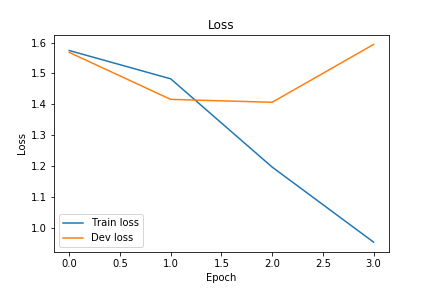
\includegraphics[width=.48\textwidth]{plot_loss.png}
    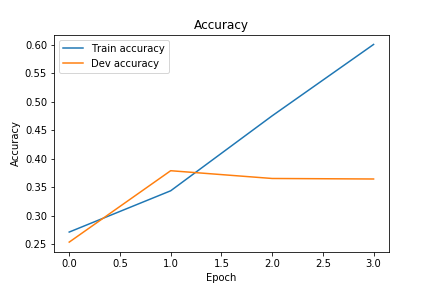
\includegraphics[width=.48\textwidth]{plot_acc.png}
    \caption{Loss and accuracy w.r.t. the number of epochs.}
    \label{fig:loss-acc}
\end{figure}
\end{solution}

\begin{question}
Be creative: use another encoder. Make it work! What are your motivations for using this other model?
\end{question}

\begin{solution}
Besides using a LSTM, we also use a 1D CNN formed by one convolutional layer and one max pooling layer. This enables the network to learn some invariant features for each class and thus yields better performance.
\end{solution}

\section{Sending your answers}

You should create a \texttt{.zip} file, named \texttt{nlp\_familyname\_firstname.zip} and send it to \texttt{vincent.lepetit@enpc.fr}. The \texttt{.zip} file should contain:
\begin{itemize}
    \item \texttt{answers.pdf} (with your answers to the questions above)
    
    \item \texttt{nlp\_project.ipynb}
    
    \item \texttt{logreg\_bow\_y\_test\_sst.txt} and \texttt{XXX\_bow\_y\_test\_sst.txt}
    
    \item \texttt{logreg\_lstm\_y\_test\_sst.txt} and \texttt{XXX\_XXX\_y\_test\_sst.txt}
\end{itemize}

Please consider that having the same format for all the students save TAs a lot of time. We will consider penalties for submissions that do not follow these simple rules. Thanks! \\

For any questions please send an email to \texttt{louismartin@fb.com}.

\end{document}
